\documentclass[nocopyrightspace]{sigchi}

% Use this command to override the default ACM copyright statement (e.g. for preprints).
% Consult the conference website for the camera-ready copyright statement.

% Arabic page numbers for submission.
% Remove this line to eliminate page numbers for the camera ready copy
% \pagenumbering{arabic}


% Load basic packages
\usepackage{balance}  % to better equalize the last page
\usepackage{graphics} % for EPS, load graphicx instead
\usepackage{times}    % comment if you want LaTeX's default font
\usepackage{url}      % llt: nicely formatted URLs

% llt: Define a global style for URLs, rather that the default one
\makeatletter
\def\url@leostyle{%
  \@ifundefined{selectfont}{\def\UrlFont{\sf}}{\def\UrlFont{\small\bf\ttfamily}}}
\makeatother
\urlstyle{leo}


% To make various LaTeX processors do the right thing with page size.
\def\pprw{8.5in}
\def\pprh{11in}
\special{papersize=\pprw,\pprh}
\setlength{\paperwidth}{\pprw}
\setlength{\paperheight}{\pprh}
\setlength{\pdfpagewidth}{\pprw}
\setlength{\pdfpageheight}{\pprh}

% Make sure hyperref comes last of your loaded packages,
% to give it a fighting chance of not being over-written,
% since its job is to redefine many LaTeX commands.
\usepackage[pdftex]{hyperref}
\hypersetup{
pdftitle={SIGCHI Conference Proceedings Format},
pdfauthor={LaTeX},
pdfkeywords={SIGCHI, proceedings, archival format},
bookmarksnumbered,
pdfstartview={FitH},
colorlinks,
citecolor=black,
filecolor=black,
linkcolor=black,
urlcolor=black,
breaklinks=true,
}

% create a shortcut to typeset table headings
\newcommand\tabhead[1]{\small\textbf{#1}}


% End of preamble. Here it comes the document.
\begin{document}

\title{Eliminating Buffer Overflows in MOOC Labs by Visualizing Memory Accesses in Parallel Programs}

\numberofauthors{3}
\author{
  \alignauthor Abdul Dakkak\\
    \affaddr{University of Illinois at Urbana-Champaign}\\
    \email{dakkak@illinois.edu}
    }

\maketitle

\begin{abstract}
  The recent popularity of Massive Open On-line Courses (MOOC) creates
  both opportunities and challenges. Since while the courses do reach
  thousands of students, systems and processes designed to deal with
  hundreds fail to scale. In the ``Hetrogenous Parallel Programming" class
  offered through Coursera, the main issue in scaling was system reliability due
  to memory indexing error encountered while running students' code.
  Since students' code is run on Graphical Processing Units (GPUs), the system
  would crash when executing certain memory errors. Aside from redundancy to avoid
  single points of failure, giving students' tools to visualize how their code
  indexes memory would not only decrease the amount of faulty code executing on
  the GPU, but also allow students' to visually understand code.
  In this project we developed Jaster: a source-to-source compiler that takes
  CUDA (a GPU programming language) as input and produces JavaScript code.
  Unlike CUDA code, which requires
  specialized GPU hardware, the JavaScript code is executed
  in the student's browser. During the JavaScript code execution, a visualization
  of the memory region is displayed along with it's access pattern.
  Since CUDA memory accesses are linearized, the tool makes use of source code
  classication to reconstruct the unlinearized access.
  The tool will be deployed in the course's next installment in January 2015.
\end{abstract}

% \keywords{Visualization; debugging; MOOC; Parallel Programming; CUDA; GPGPU; }

\section{Introduction}


With the expantion of the reach of programming courses through Massive Open Online Courses,
educators are rethinking the way these courses are offered. The expectation that a 
student would setup a development environment (setting a compiler, learning 
new tools for debugging, and setting up an IDE) would limit the reach of the course, since
it would exclude people who cannot install such software or cannot afford it. 
Futhermore, it requires at least a week for students to orient themselves with the 
new flow, which is long for the relatively short courses.
Thus multiple courses now offer a way to how on the problem through web interfaces.

The trend is not limitated to educators. Microsoft~\cite{1_visualstudio.com_2014} and Eclipse~\cite{orion} both have an online
version of their IDE and compiler. Similarly, most languages now offer a playground area
where users can post and evaluate code.

All of these systems assume that you are running generic code, but what if you'd like
to teach a course that requires special hardware. Furthremore, the hardware cannot be
emulated. This was the challenge faced when we setup the Coursera Hetrogenous Parallel
Programming course. We would like users to have as much control while still maintaining
availability and fairness\footnote{The system is live today at {\tt webgpu.hwu.crhc.illinois.edu}}. 

Based on user's surveys the most common complain is the limited number of developer tools
offered through the site. In this project we develop a tool to visualize how a CUDA
program executes and how memory is addressed. We first write a traslator from 
CUDA to JavaScript that maintains the original semantics.
We classify labs from previous iterations of the course, which contain the most
common techniques for CUDA execution and 
memory addressing. Then, given a buggy peice of code we find the closest lab to 
not only determine how to layout the visualization, but also determine the 
unlinearlized memory access.
An overview of our pipeline is show in figure~\ref{fig:pipeline}.

\begin{figure}[!h]
\centering
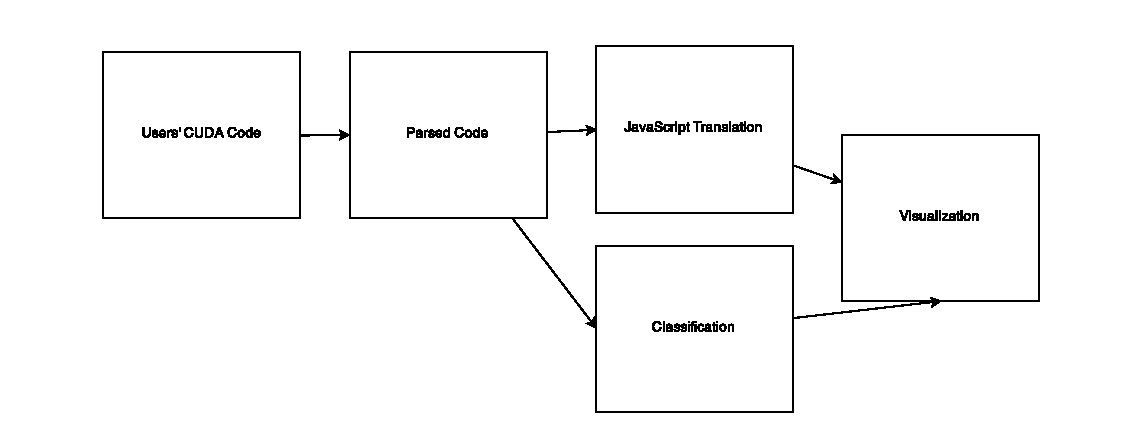
\includegraphics[width=0.9\columnwidth]{flow}
\caption{The pipeline of our project. In this flow code is first
parsed, transcompiled, classified, and then visualized.}
\label{fig:pipeline}
\end{figure}

\subsection{Previous Work}


Due to the fact we think sequentially, parallel programming is hard to get
right. A slew of other problems crop up due to the  indeterministic nature of
parallel code. Logic errors such as race conditions, deadlocks, and starvation
cause indeterministicly generate unexpected outcome or cause system errors.
Since parallel languages are also hosted within a low level language,
you inherit aditional problems such as: unsafe type casts, buffer overflows,
bad array index calculations. The variety of these bugs makes courses such 
as HPP not approcahable for sutdents who do not percervere for the first few 
weeks.


Current CUDA debugging tools such as Nsight for Visual Studio or {\tt cuda-gdb}
for Unix operate by suspending the GPU. This means that one needs at least two
GPU cards are needed while debugging GPU code. Futhremore, these debugging tools
are quite involved --- requiring the learning of new commands, understand a
different workflow, and because these tools are proprietery cannot not be easily
integrated with the course's system.


Other than low level debugging tools, we are not aware of any work on 
to visualize CUDA program execution --- and certainly not one that 
does so by transpiling CUDA to JavaScript.



\section{C++ Parser}

The first is a C++ library the uses CLANG RecursiveAST~\cite{lattner2004llvm} interface to parse CUDA code
and storing the Abstract Syntax Tree (AST) nodes in a mutable representation
We developed a new AST interface, since the one provided by CLANG is immutable.
Our AST interface stores not only the node information, but also the location
of the code within the input file, the text underlying the node, and parent child
relashionship. Once the parsing is complete, our datastructure dumps the information
into JSON form. A C++ expression such as {\tt x + 1} generates the following JSON
output:

\begin{verbatim}
  {
    type: "BinaryExpression",
    operator: "*",
    left: {
      type: "Identifier",
      name: "x",
      loc: {
        start: { line: 2, column: 8 },
        end:   { line: 2, column: 9 }
      }
    },
    right: {
      type: "Literal",
      value: 1,
      loc: {
        start: { line: 2, column: 10 },
        end:   { line: 2, column: 11 }
      }
    }
  }
\end{verbatim}

We use the Mozzila AST specification, to name the fields within the JSON datastructure.
While not a standard, it is the only documented JavaScript AST serialization specification
that we are aware of. Futhermore, tools to read, verify, and traverse the AST in the
Mozilla Specification exist.

Even though the input source code might not be parsable as CUDA code without macro expantion,
our tool performs the macro expansion but generates the source mapping to the original 
unprocessed text.


\section{JavaScript Transpiler}

The JavaScript source-to-source compiler can be divided into multiple steps.
First, code must maintain the same type meaning --- even though JavaScript 
is dynamically typed, second it must be performant, finally it must contain
enought meta data to backtrack to the original input program.

\subsection{Pointer Types in JavaScript}

Since JavaScript does not contain type information, and types are needed to
properly maintain the semantics of C++ --- such as truncation of floats when
assigned to integers or offset calculation for array indexing. The transpiler
adds type information in the {\tt functionStack\$} type field. Code such as
{\tt int x = 1.2;} results in the following JavaScript code

\begin{verbatim}
  functionStack$['x'] = Math.floor(1.2);
  lib.setType(functionStack$, 'x', {
    type: 'TypeExpression',
    addressSpace: [''],
    qualifiers: [],
    bases: ['int']
  });
\end{verbatim}

The type information is queried when calculating the offset in the heap when
indexing an array. For example, for code such as

\begin{verbatim}
  int * y;
  double * x;
  ....
  x[2] = 5 + y[1];
\end{verbatim}

then the element size of the array {\tt y} is $\mathtt{sizeof(int)} = 4$.
So, {\tt y[1]} causes $4$ bytes to be read from index $4$ of {\tt y} and
interpreted as an integer. Similarly, $\mathtt{sizeof(double)} = 8$ bytes
must be set at index $2 * \mathtt{sizeof(double)} = 16$ from array {\tt x}
as a double precision number.


\section{Runtime}

Several design decisions in the runtime were influenced by the limitations
of current JavaScript engines~\cite{vilk2014doppio,vouillon2013bytecode,zakai2011emscripten}.
We try to make use as much of the newer JavaScript features as possible that are
able to achieve good performance, while still maintaing shims to allow us
to support older browers. The runtime therefore makes heavy use of WebWorkers~\cite{green2012web}, 
TypedArrays~\cite{matsakistyped, grimmer2014efficient}, promises~\cite{kambona2013evaluation,bonetta2013tigerquoll},
and generators in our implementation. 

\subsection{C++ Types}

JavaScript contains only one literal numeric type: an IEEE double 
precision double. To emulate the other types in JavaScript effiently we
again use TypedArrays since they are able to represent 8, 16, and 32 bit
signed and unsigned integers. Scalar C++ operations on these types get
translated as operations on a 1 element array of the corresponding type.
To emulate 64 bit integers, we use two 32 bit integers and perform the
high and low bit calculation~\cite{warren2013hacker}.
We experimented with other ways of emulating 64bit integers, but found 
using 32bits was the most efficient.

\subsection{The C++ Heap}

We use TypedArrays to model the C++ Heap. This is now a common technique 
when transpiling from unmanaged languages. At the initialization of the 
program, then runtime allocates a slab of memory. This memory is then
used as a pool where allocations are honored by taking a slab of the 
buffer.

Since CUDA memory is in a different address space than the host memory,
the runtime creates two heaps. Errors are thrown if operations done on
the allocated memory result in undefined behavior (operating on GPU
memory using host memory functions for example).

\subsection{CUDA Execution}


We use a combination of asynchonus operations and true multithreading
to simulate CUDA execution. The code kernel invocations are dispatched
into a thread pool. Each thread pool then invokes a collection in a 
round robin way generating a promise. Only when the promises are fulfilled
between all the threads can program continue execution. By performing
this technique we do not perform any blocking operation on the main UI
thread.

Since JavaScript threads cannot share data, we develope a communication
language between threads and the master thread (which has the data). A
thread requesting data from global memory generates a message which the
master thread corresponds to. Effectively we translate the shared threaded
execution model to a message passing actor model.

\subsection{Performance}

When trying to emulate the exeution of GPU code, one must observe that GPUs
are well suited for the types of labs in the HPP MOOC and that CUDA is a 
low level programming language. Given that JavaScript is dynamically typed,
we make use of a lot of performance oprtunities afforeded to us by the standard.
We use TypedArrays~\cite{guha2010essence,maffeis2008operational} to emulate the heap,
for example, while webworkers are used
to make use of multiple threads of execution.

By creating artificial boundaries within functions, we are able to schedule
the code to run on the main thread while maintaining the UI's responsiveness.
Furthremore, we store all stack information in a special variable which 
allows us pause and resume the execution frame at any point.

To maintain the same execution time as CUDA, we rescale the inputs to be a
tenth of the size of data that is traditionally given for lab execution.



\section{Code Similarity}

Since template code was provided to the students, and the code follows the course
lectures, structural similarity within the solutions should be common. To hone in
on the visualization, we mine the dataset (which contains a sampling of 100 programs
from each lab picked from compilable programs in a  from over 2 million program
database~\footnote{We are limited to a small set of programs because
of the computational complexity of the algorithm. In the comming weeks we plan on
we plan on performing full correlation between the codes. since
the code similarity algorithm is computationally expensive}.

We use the Zhang-Shasha~\cite{zhang1989simple} algorithm measure the distance between two trees with respect to
distance functions. The algorithm complexity is $O(n^4)$ in time and $O(n^2)$ in space, but
that's midigated by the fact that this computation is done on the client's machine.
Zhang-Shasha's algorithm determines the distance between two pairs of ASTs by
calculating the number of insersions, deletions, and renaming of the nodes
required to equate the AST nodes. Since two noes might be different in the AST but semantically
the same, we perform canonicalization to mimic semantic equivalence. Since we still want
to be able to present the user with the AST differences, we maintain the original node
information while performing the canonicalization.

\subsubsection{Cannonicalization of the AST Representation}

Because of the high complexity, we prune the tree to only include the CUDA kernel part.
Since two codes might have different AST representation but same semantic meaning,
we perform a normalization step on the AST before computing the distance.
We first replace all the identifiers with a canonical name. Identifiers that are not within
the body of the function are deleted, since they are given as part of the template code.
Identifiers within the function body are computed based on
a hash of how the identifier is assigned to within the code.
Literals (such as integers) are ignored since they do not contribute to any structural
difference in the code (they do contribute to the hash calculation for the identifiers however).
{\tt for} and {\tt do} while loops are rewritten to their {\tt while} representation,
conditional expressions (expressions of the form {\tt var = cond ? then : else }) are rewritten
to {\tt if (cond) \{ var = then; \} else \{ var = else; \}},
{\tt if} conditions are rewritten so that the biggest node is within the {\tt then} branch
of the condition. Finally, for compound expressions are canonicallize the code based on the
following rewrite rules:

\begin{itemize}
  \item Types of variable declarations are removed : statements such as {\tt int x = 4;}
  are replaced wth {\tt x = 4;}
  \item Non-side effecting statements are pruned : statements are {\tt x;} or {\tt f();} where
  {\tt f} is known to be a pure function get pruned
  \item Compound binary expressions are reordered based on operator precidence:
  $a \, \mathtt{op}_1  (b \, \mathtt{op}_2 \, c) \rightarrow (b \, \mathtt{op}_2 \, c) \, \mathtt{op}_1 \, a$
  iff $\mathtt{op}_2$ has lower precidence than $\mathtt{op}_1$
  \item Leaf binary operations are reordered based on the lexographical ordering
  of the leafs :
  $a \, \mathtt{op} \, b \rightarrow b \, \mathtt{op} \, a$ iff $b$ is lexographically less than $a$
  \item Strength reduction is applied : expressions such as {\tt x * 2} get replaced by {\tt x << 1} or
  {\tt x * 1 = x}.
  \item Constant propagation is applied : expressions such as {\tt a = 3; b = a * 4;} get replaced
  by {\tt a = 3; b = 12;}
\end{itemize}

To lexographically order the AST leaf node we use the follwing heuristic:
literals of the same type use the $<$ operation for ordering,
literals of different types are first ordered based on their value and then,
in case of a tie, the tie is broken by considering the bytesize of the types,
literal nodes are always lexographically less than identifiers,
and identifiers use string lexographical ordering.

In cases where a compound node cannot be canonicallized, we mark the node for
special processing during the distance calculation. During computation, the edit
distance of these nodes is computed as the minimum distance of its children.

When computing the edit distance, the cost for replacement of an identifier is
proportional to the Levenshtein distance of strings. Deletion and insersions
contribute 1 to the cost.

\subsubsection{Zhang-Shasha Tree Edit Distance}



\subsection{Memory Access Similarity}



\section{FrontEnd Implementation}

We use React~\cite{reynders2014multi} to implement our visualization.
React constructs a virtual DOM and only performs DOM updates when
the tree is different enough from the one being displayed. 
By having batched rendering, versus fragmented ones, we 
were able to achive good performance over a pure SVG based 
rendering.

Furthremore, by having each thread be a react component, our code
is very simple to reason about. React also provides good binding 
between the data and visual elements. Changing the data in 
one of it's components triggers a rerendering of that component.
If a component has children, then all of the children may get
rerendered as well.

React also contains Mixins to memoize some rendering. If a 
component is requested to be redrawn, then React can ignore 
that request if it can show that the compoent data did not 
mutate.


\section{Results}



\section{Limitations}

\section{Future Work}

\bibliographystyle{acm-sigchi}
\bibliography{sample}
\end{document}
